
    \documentclass{article}
    \usepackage{graphicx}
    \usepackage{booktabs}
    \usepackage{pgfplots}
    \pgfplotsset{compat=1.17}
    \begin{document}

    \title{Custom Analysis Report}
    \author{Generated by Streamlit}
    \date{\today}
    \maketitle

    \section{Overall Summary Statistics}
    \begin{tabular}{ll}
    \toprule
    Metric & Value \\
    \midrule
    Total Programs & 28443.0 \\ 
Programs with Weight 1 & 28402.0 \\ 
Programs with Weight 500 & 41.0 \\ 
Average Operations Count & 51.48082129170622 \\ 
Average Variables Count & 137.63098126076716 \\ 
Average Cyclomatic Complexity & 1.0 \\ 
Average Operations Count Weight 1 & 51.4955636926977 \\ 
Average Variables Count Weight 1 & 137.6701288641645 \\ 
Average Cyclomatic Complexity Weight 1 & 1.0 \\ 
Average Operations Count Weight 500 & 41.26829268292683 \\ 
Average Variables Count Weight 500 & 110.51219512195122 \\ 
Average Cyclomatic Complexity Weight 500 & 1.0 \\ 

    \bottomrule
    \end{tabular}

    \section{Grouped Operation Statistics by Category}
    \begin{tabular}{llllll}
    \toprule
    Category & Description & 1 Count & 500 Count & 1 Mean & 500 Mean \\
    \midrule
    Arithmetic and Logical Operations & Operations performing arithmetic or logical manipulations. & 73202 & 69 & 0.644338426871347 & 0.42073170731707316 \\ 
Class Definitions & Operations related to defining classes. & 158035 & 190 & 0.1686127524096681 & 0.14042867701404288 \\ 
Comparison Operations & Operations that perform comparisons. & 16789 & 16 & 0.197040114545924 & 0.13008130081300814 \\ 
Conditional Operations & Operations for conditional evaluations. & 1023 & 0 & 0.03601859024012394 & 0.0 \\ 
Control Flow Statements & Statements that alter the flow of control in the program. & 50729 & 51 & 0.04465266530526019 & 0.031097560975609756 \\ 
Exception Handling & Operations for handling exceptions. & 179 & 0 & 0.0063023730723188506 & 0.0 \\ 
Function Calls & Operations for calling functions. & 42861 & 49 & 0.7545419336666432 & 0.5975609756097562 \\ 
Function Definitions & Operations related to defining functions. & 100222 & 116 & 0.2714380894086549 & 0.21763602251407127 \\ 
Load Operations & Operations related to loading values into variables. & 425577 & 492 & 1.248670868248715 & 1.0 \\ 
Method Calls & Operations for calling methods of objects. & 49114 & 61 & 0.288207403234514 & 0.24796747967479674 \\ 
Object Operations & Operations related to creating and manipulating objects. & 419716 & 520 & 0.591107668474051 & 0.5073170731707317 \\ 
Property Operations & Operations on properties of objects. & 114398 & 113 & 0.19180071155284167 & 0.13124274099883854 \\ 
String Operations & Operations related to manipulating strings. & 1716 & 4 & 0.020139426800929512 & 0.032520325203252036 \\ 
Type Checking Operations & Operations for checking the type of variables. & 1334 & 2 & 0.04696852334342652 & 0.04878048780487805 \\ 
Variable Declarations & Operations for declaring variables. & 7682 & 9 & 0.09015797009600263 & 0.07317073170731707 \\ 

    \bottomrule
    \end{tabular}

    \section{Comparison of Averages by Category}
    \begin{tikzpicture}
    \begin{axis}[
        width=1.5\textwidth,
        height=0.8\textheight,
        xlabel={Operation Category},
        ylabel={Average Count},
        xtick={1, 2, 3, 4, 5, 6, 7, 8, 9, 10, 11, 12, 13, 14, 15},
        xticklabels={{Arithmetic and Logical Operations}, {Class Definitions}, {Comparison Operations}, {Conditional Operations}, {Control Flow Statements}, {Exception Handling}, {Function Calls}, {Function Definitions}, {Load Operations}, {Method Calls}, {Object Operations}, {Property Operations}, {String Operations}, {Type Checking Operations}, {Variable Declarations}},
        ymajorgrids=true,
        grid style=dashed,
        x tick label style={rotate=90, anchor=east},
    ]
    
    \addplot[
        ybar,
        bar width=.4cm,
        fill=blue,
        draw=blue,
        mark=none,
    ] coordinates {(1, 0.644338426871347) (2, 0.1686127524096681) (3, 0.197040114545924) (4, 0.03601859024012394) (5, 0.04465266530526019) (6, 0.0063023730723188506) (7, 0.7545419336666432) (8, 0.2714380894086549) (9, 1.248670868248715) (10, 0.288207403234514) (11, 0.591107668474051) (12, 0.19180071155284167) (13, 0.020139426800929512) (14, 0.04696852334342652) (15, 0.09015797009600263) };

    \addplot[
        ybar,
        bar width=.4cm,
        fill=red,
        draw=red,
        mark=none,
    ] coordinates {(1, 0.42073170731707316) (2, 0.14042867701404288) (3, 0.13008130081300814) (4, 0.0) (5, 0.031097560975609756) (6, 0.0) (7, 0.5975609756097562) (8, 0.21763602251407127) (9, 1.0) (10, 0.24796747967479674) (11, 0.5073170731707317) (12, 0.13124274099883854) (13, 0.032520325203252036) (14, 0.04878048780487805) (15, 0.07317073170731707) };
    
    \legend{Fuzzilli's Programs, JSTargetFuzzer's Programs}
    \end{axis}
    \end{tikzpicture}

    \end{document}
    